\paragraph{Comparativas}

En esta sección se presenta una comparativa preliminar del conjunto de funciones presentado junto con sus versiones de dos y cuatro fuentes. 

\begin{itemize}
    \item \textbf{A. Comparación por número de fuentes}

En la literatura del recurso que presenta la arquitectura del modelo utilizado en este proyecto se comentan en múltiples ocasiones las diferencias entre estos dos enfoques al problema.
La separación que resulta en el conjunto de dos fuentes, ya visto en las primeras versiones del entrenamiento, es un enfoque más sencillo que permite una "binarización" (se puede reducir el problema a identificar el elemento de las vocales y lo que no sea vocales agruparlo en acompañamiento) del problema al reducirse a dos salidas.
4 stems obliga a estimar más fuentes que pueden solaparse espectralmente; por ello se espera una tarea más difícil, y los resultados finales permiten comprobarlo.

De manera adicional se realizó un análisis exploratorio de los valores SDR y SNR agrupados por género musical, mostrado en la Figura \ref{fig:SNR SDR by genre}. Este análisis tiene únicamente carácter descriptivo, ya que el subconjunto utilizado no fue diseñado mediante un muestreo estratificado por género y el número de pistas disponible para cada categoría es limitado. Por tanto, las diferencias observadas no permiten establecer relaciones causales entre un género musical concreto y la dificultad de separación, aunque resultan útiles para visualizar la variabilidad de comportamiento del sistema entre pistas con características diferentes.

\begin{figure}[H]
    \begin{center}
    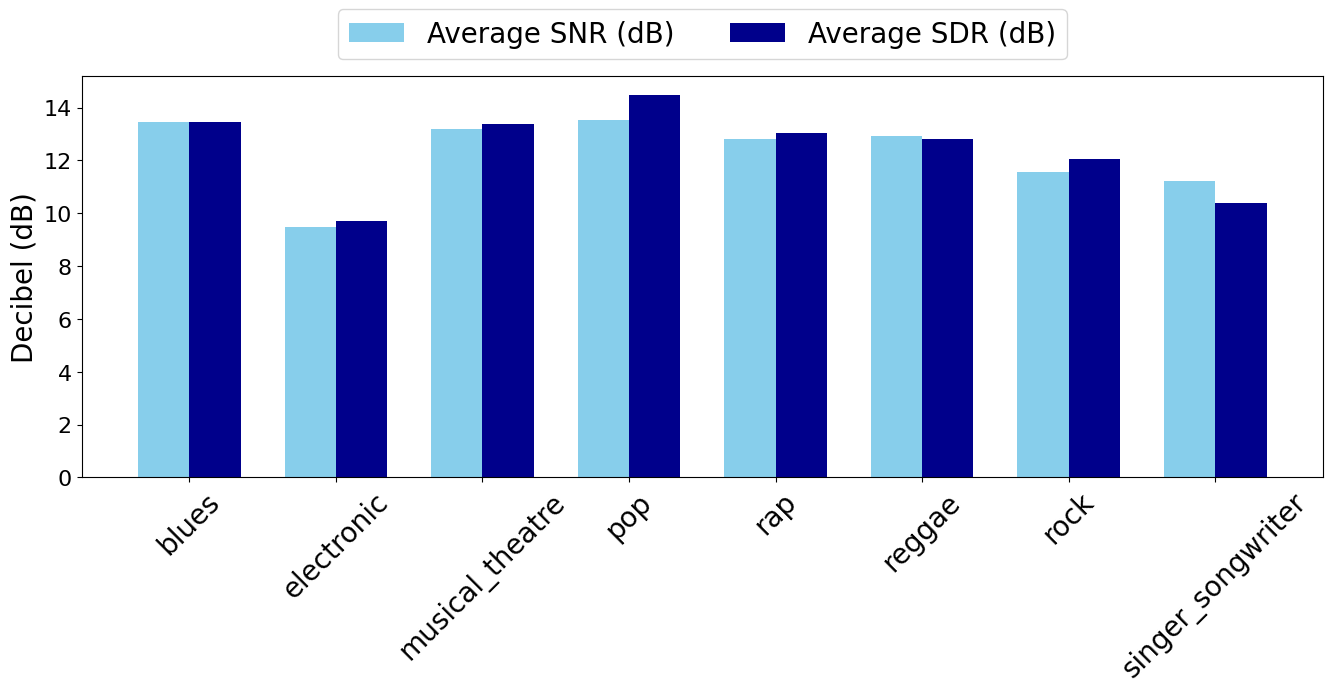
\includegraphics[width=0.7\textwidth]{commons/Fig10.png}
    \caption{Media de métricas SDR y SNR por género musical en cuatro fuentes.}
    \label{fig:SNR SDR by genre}
    \end{center}
\end{figure}

    \item \textbf{B. Comparación por familia de pérdida}

Se han agrupado las funciones de pérdida por las familias aritméticas a las que pertenecen por su naturaleza:

    \begin{itemize}
        \item Pérdidas de magnitud directa: L1 , L2.
        \item Pérdidas frecuenciales: L1\_freq, L2\_freq.
        \item Pérdidas logarítmicas: logL1, logL2, log\_mag, log\_compressed\_l2.
        \item Pérdidas informadas por fase o potencia: LPSA, lpsa\_phase.
        \item Pérdidas basadas en máscara: mask\_l1
        \item Pérdidas experimentales: deep\_feature , deep\_feature\_emd
    \end{itemize}

Las distintas familias de pérdidas introducen sesgos de entrenamiento diferentes.
Las pérdidas en escala logarítmica trabajan sobre una representación comprimida de la magnitud espectral, ya que la aplicación del logaritmo reduce el rango dinámico del espectrograma \cite{yang2021dprtf}. Esto modifica el peso relativo de los errores, evitando que los bins de mayor energía dominen completamente la optimización.
Las pérdidas frecuenciales comparan directamente estimaciones y referencias en el dominio tiempo-frecuencia, normalmente mediante distancias punto a punto entre espectrogramas \cite{sahai2019spectrogram}. 
Por su parte, las pérdidas basadas en máscara emplean como objetivo una máscara ideal o aproximada, guiando al modelo hacia una asignación explícita, aunque generalmente suave, de los bins tiempo-frecuencia a las distintas fuentes \cite{xia2017optimalratio,wang2008tfmasking}.

\end{itemize}